\begin{figure}
    \centering

    \tikzset{every picture/.style={line width=0.75pt}} %set default line width to 0.75pt        

    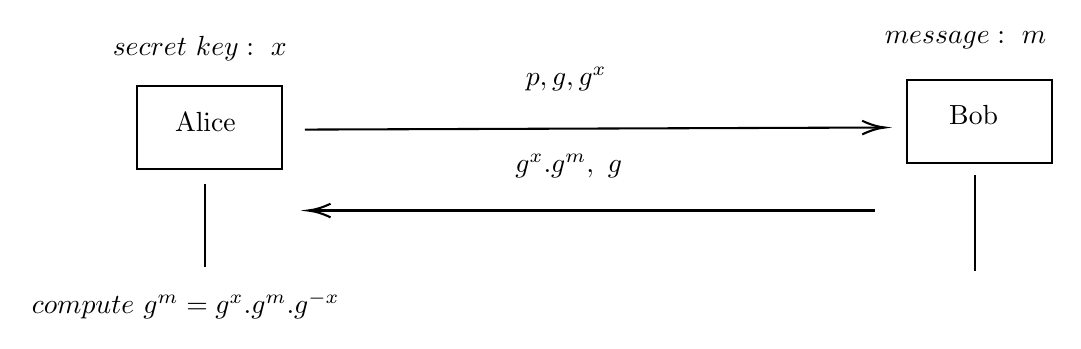
\begin{tikzpicture}[x=0.75pt,y=0.75pt,yscale=-1,xscale=1]
    %uncomment if require: \path (0,181); %set diagram left start at 0, and has height of 181

    %Shape: Rectangle [id:dp22737212763642367] 
    \draw   (95,32) -- (165,32) -- (165,72) -- (95,72) -- cycle ;

    %Shape: Rectangle [id:dp5854265454101574] 
    \draw   (466,29) -- (536,29) -- (536,69) -- (466,69) -- cycle ;

    %Straight Lines [id:da2877686107509583] 
    \draw    (176,53) -- (453.5,52.01) ;
    \draw [shift={(455.5,52)}, rotate = 179.8] [color={rgb, 255:red, 0; green, 0; blue, 0 }  ][line width=0.75]    (10.93,-3.29) .. controls (6.95,-1.4) and (3.31,-0.3) .. (0,0) .. controls (3.31,0.3) and (6.95,1.4) .. (10.93,3.29)   ;
    %Straight Lines [id:da7116831290080069] 
    \draw    (128,79) -- (128,119) ;
    %Straight Lines [id:da19342470100111897] 
    \draw    (499,75) -- (499,121) ;
    %Straight Lines [id:da2580219434326909] 
    \draw    (450.5,92) -- (179.5,92) ;
    \draw [shift={(177.5,92)}, rotate = 360] [color={rgb, 255:red, 0; green, 0; blue, 0 }  ][line width=0.75]    (10.93,-3.29) .. controls (6.95,-1.4) and (3.31,-0.3) .. (0,0) .. controls (3.31,0.3) and (6.95,1.4) .. (10.93,3.29)   ;

    % Text Node
    \draw (112,43) node [anchor=north west][inner sep=0.75pt]   [align=left] {Alice};
    % Text Node
    \draw (485,40) node [anchor=north west][inner sep=0.75pt]   [align=left] {Bob};
    % Text Node
    \draw (281,21.4) node [anchor=north west][inner sep=0.75pt]    {$p,g,g^{x}$};
    % Text Node
    \draw (276,63.4) node [anchor=north west][inner sep=0.75pt]    {$g^{x} .g^{m} ,\ g$};
    % Text Node
    \draw (82,6.4) node [anchor=north west][inner sep=0.75pt]    {$secret\ key:\ x$};
    % Text Node
    \draw (454,4.4) node [anchor=north west][inner sep=0.75pt]    {$message:\ m$};
    % Text Node
    \draw (43,129.4) node [anchor=north west][inner sep=0.75pt]    {$compute\ g^{m} =g^{x} .g^{m} .g^{-x}$};

    \end{tikzpicture}

    \caption{New encryption scheme}\label{fig:nisec_scheme}
\end{figure}

\subsection*{a) Drawbacks of the new encryption scheme}
%
\begin{itemize}
    \item \textbf{Lack of data integrity}: HMAC should be implemented on top of the
    public parammeters to make sure they were not intercepted.
    \item \textbf{Lack of mutual authentication}: there is no authentication protocol between
    the sender and the receiver, so it very easy for an attacker to intervene the 
    connection.
    \item \textbf{Resource expensive algorithms}: using public key cryptography to
    encrypt/decrypt the long message takes lots of time and computational
    resources. Instead, symmetric cryptography should be used to avoid 
    operating on enormous prime numbers. The asymmetric cryptography, public key
    cryptography, can be used to encrypt the symmetric key. Then the encrypted
    key is utilized to encrypt/decrypt a long message (a large file).
\end{itemize}

Some possible attacks:

\begin{figure}
    \centering

    \tikzset{every picture/.style={line width=0.75pt}} %set default line width to 0.75pt        

    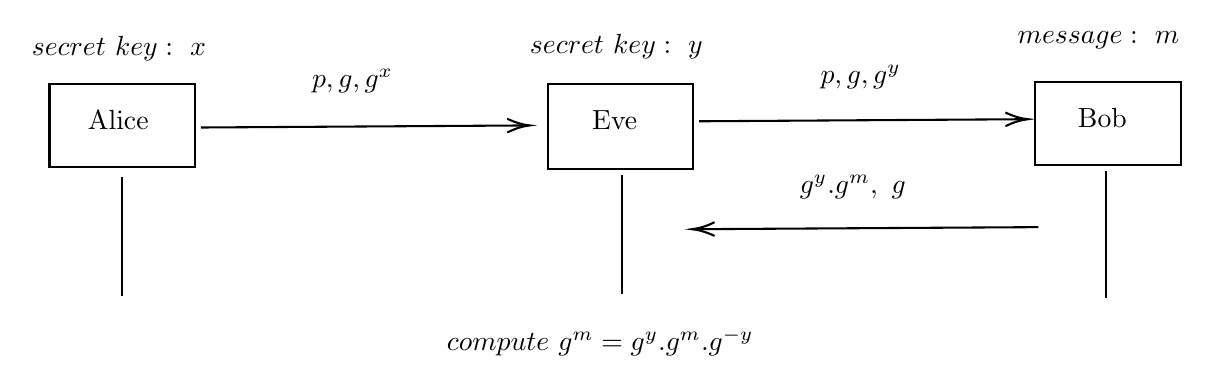
\begin{tikzpicture}[x=0.75pt,y=0.75pt,yscale=-1,xscale=1]
    %uncomment if require: \path (0,234); %set diagram left start at 0, and has height of 234

    %Shape: Rectangle [id:dp6501223431872357] 
    \draw   (54,70) -- (124,70) -- (124,110) -- (54,110) -- cycle ;

    %Shape: Rectangle [id:dp8447479220950903] 
    \draw   (529,69) -- (599,69) -- (599,109) -- (529,109) -- cycle ;

    %Straight Lines [id:da3587916713070962] 
    \draw    (127,91) -- (283.5,90.01) ;
    \draw [shift={(285.5,90)}, rotate = 179.64] [color={rgb, 255:red, 0; green, 0; blue, 0 }  ][line width=0.75]    (10.93,-3.29) .. controls (6.95,-1.4) and (3.31,-0.3) .. (0,0) .. controls (3.31,0.3) and (6.95,1.4) .. (10.93,3.29)   ;
    %Straight Lines [id:da12630867495123377] 
    \draw    (89,115) -- (89,172) ;
    %Straight Lines [id:da07235943303271719] 
    \draw    (563,112) -- (563,173) ;
    %Straight Lines [id:da044820189761365814] 
    \draw    (530.5,139) -- (365.5,139.99) ;
    \draw [shift={(363.5,140)}, rotate = 359.66] [color={rgb, 255:red, 0; green, 0; blue, 0 }  ][line width=0.75]    (10.93,-3.29) .. controls (6.95,-1.4) and (3.31,-0.3) .. (0,0) .. controls (3.31,0.3) and (6.95,1.4) .. (10.93,3.29)   ;
    %Shape: Rectangle [id:dp8175805944937183] 
    \draw   (294,70) -- (364,70) -- (364,111) -- (294,111) -- cycle ;

    %Straight Lines [id:da4400636896192306] 
    \draw    (367,88) -- (523.5,87.01) ;
    \draw [shift={(525.5,87)}, rotate = 179.64] [color={rgb, 255:red, 0; green, 0; blue, 0 }  ][line width=0.75]    (10.93,-3.29) .. controls (6.95,-1.4) and (3.31,-0.3) .. (0,0) .. controls (3.31,0.3) and (6.95,1.4) .. (10.93,3.29)   ;
    %Straight Lines [id:da8522907791652553] 
    \draw    (330,114) -- (330,171) ;

    % Text Node
    \draw (179,61.4) node [anchor=north west][inner sep=0.75pt]    {$p,g,g^{x}$};
    % Text Node
    \draw (414,112.4) node [anchor=north west][inner sep=0.75pt]    {$g^{y} .g^{m} ,\ g$};
    % Text Node
    \draw (44,45.4) node [anchor=north west][inner sep=0.75pt]    {$secret\ key:\ x$};
    % Text Node
    \draw (519,43.4) node [anchor=north west][inner sep=0.75pt]    {$message:\ m$};
    % Text Node
    \draw (244,186.4) node [anchor=north west][inner sep=0.75pt]    {$compute\ g^{m} =g^{y} .g^{m} .g^{-y}$};
    % Text Node
    \draw (548,80) node [anchor=north west][inner sep=0.75pt]   [align=left] {Bob};
    % Text Node
    \draw (71,81) node [anchor=north west][inner sep=0.75pt]   [align=left] {Alice};
    % Text Node
    \draw (314,81.49) node [anchor=north west][inner sep=0.75pt]   [align=left] {Eve};
    % Text Node
    \draw (424,59.4) node [anchor=north west][inner sep=0.75pt]    {$p,g,g^{y}$};
    % Text Node
    \draw (284,44.4) node [anchor=north west][inner sep=0.75pt]    {$secret\ key:\ y$};

    \end{tikzpicture}

    \caption{The attacker impersonates the receiver}\label{fig:imp_receiver}
\end{figure}

\begin{figure}
    \centering


    \tikzset{every picture/.style={line width=0.75pt}} %set default line width to 0.75pt        

    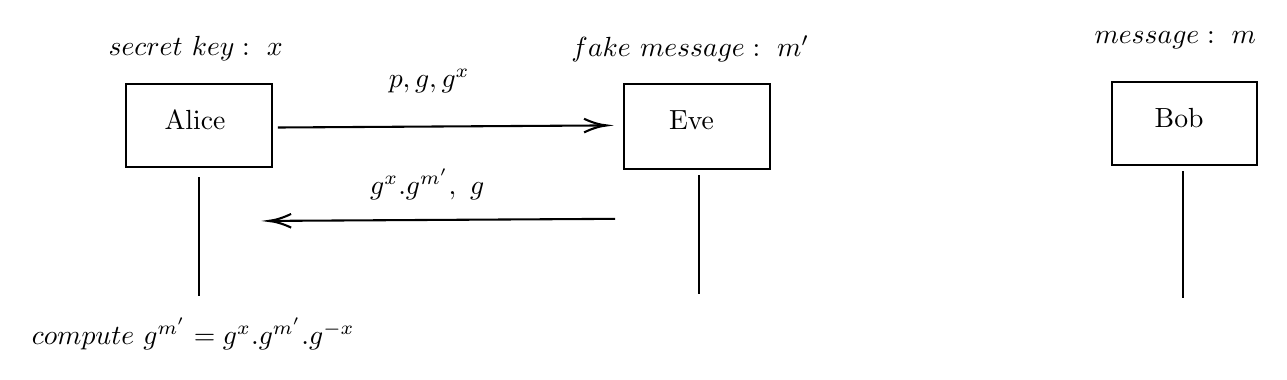
\begin{tikzpicture}[x=0.75pt,y=0.75pt,yscale=-1,xscale=1]
    %uncomment if require: \path (0,300); %set diagram left start at 0, and has height of 300

    %Shape: Rectangle [id:dp1403171227510649] 
    \draw   (74,90) -- (144,90) -- (144,130) -- (74,130) -- cycle ;

    %Shape: Rectangle [id:dp6601513404208796] 
    \draw   (549,89) -- (619,89) -- (619,129) -- (549,129) -- cycle ;

    %Straight Lines [id:da9197769654145035] 
    \draw    (147,111) -- (303.5,110.01) ;
    \draw [shift={(305.5,110)}, rotate = 179.64] [color={rgb, 255:red, 0; green, 0; blue, 0 }  ][line width=0.75]    (10.93,-3.29) .. controls (6.95,-1.4) and (3.31,-0.3) .. (0,0) .. controls (3.31,0.3) and (6.95,1.4) .. (10.93,3.29)   ;
    %Straight Lines [id:da9223813286436544] 
    \draw    (109,135) -- (109,192) ;
    %Straight Lines [id:da34247791753331325] 
    \draw    (583,132) -- (583,193) ;
    %Straight Lines [id:da7861276918756701] 
    \draw    (309.5,155) -- (144.5,155.99) ;
    \draw [shift={(142.5,156)}, rotate = 359.66] [color={rgb, 255:red, 0; green, 0; blue, 0 }  ][line width=0.75]    (10.93,-3.29) .. controls (6.95,-1.4) and (3.31,-0.3) .. (0,0) .. controls (3.31,0.3) and (6.95,1.4) .. (10.93,3.29)   ;
    %Shape: Rectangle [id:dp488004334450037] 
    \draw   (314,90) -- (384,90) -- (384,131) -- (314,131) -- cycle ;

    %Straight Lines [id:da988601175202231] 
    \draw    (350,134) -- (350,191) ;

    % Text Node
    \draw (199,81.4) node [anchor=north west][inner sep=0.75pt]    {$p,g,g^{x}$};
    % Text Node
    \draw (190,129.4) node [anchor=north west][inner sep=0.75pt]    {$g^{x} .g^{m'} ,\ g$};
    % Text Node
    \draw (64,65.4) node [anchor=north west][inner sep=0.75pt]    {$secret\ key:\ x$};
    % Text Node
    \draw (539,63.4) node [anchor=north west][inner sep=0.75pt]    {$message:\ m$};
    % Text Node
    \draw (27,201.4) node [anchor=north west][inner sep=0.75pt]    {$compute\ g^{m'} =g^{x} .g^{m'} .g^{-x}$};
    % Text Node
    \draw (287,65.4) node [anchor=north west][inner sep=0.75pt]    {$fake\ message:\ m'$};
    % Text Node
    \draw (334,101.49) node [anchor=north west][inner sep=0.75pt]   [align=left] {Eve};
    % Text Node
    \draw (568,100) node [anchor=north west][inner sep=0.75pt]   [align=left] {Bob};
    % Text Node
    \draw (91,101) node [anchor=north west][inner sep=0.75pt]   [align=left] {Alice};


    \end{tikzpicture}

    \caption{The attacker impersonates the sender}\label{fig:imp_sender}
\end{figure}

\subsection*{b) Linear cihpertext homomorphic and linear key homomorphic}
%
The notation \(Enc(pk_i, x_i)=g^{sk_i}\cdot g^{x_i}\) is used to denote the encryption of the
message \(x_i\) using the public key \(pk_i\).

\textbf{Prove that the scheme is linear ciphertext homomorphic}\\

The linear ciphertext homomorphic property is then:
\begin{align*}
    Enc(pk_1, x_1) \cdot...\cdot Enc(pk_n, x_n) &= (g^{sk_1}\cdot g^{x_1})
    \cdot...\cdot(g^{sk_n}\cdot g^{x_n})\\
    &= (g^{sk_1}\cdot...\cdot g^{sk_n})\cdot(g^{x_1}\cdot...\cdot g^{x_n})\\
    &= g^{sk_1+\cdots +sk_n}\cdot g^{x_1+\cdots +x_n}\\
    &= Enc(pk_1\cdot...\cdot pk_n, x_1+\cdots +x_n)
\end{align*}

\textbf{Prove that the scheme is linear key homomorphic}\\
Given \emph{n} public/private key pairs:\\
\begin{align*}
    (pk_1,sk_1),\cdots,(pk_n,sk_n),
\end{align*}

for each key pair the following expression holds:
\begin{align*}
    &pk_i,sk_i\\
    \Leftrightarrow &g^{sk_i},sk_i.
\end{align*}

Using a newly constructed key pair:

\begin{align*}
    &pk_1\cdot...\cdot pk_n, sk_1+...+ sk_n\\
    \Leftrightarrow &g^{sk_1}\cdot...\cdot g^{sk_n}, sk_1+...+ sk_n\\
    \Leftrightarrow &g^{sk_1+...+sk_n}, sk_1+...+sk_n.
\end{align*}

Thus, the new key pair is valid, so the linear key homomorphic property holds.

\subsection*{c) Explain how the CSP can compute \(x_1+\cdots+x_n\)}
%
The CSP already know the sum of secret keys:
\begin{align*}
    sk_1+\cdots+sk_n,
\end{align*}
and given each ciphertext \(c_i\), it can compute the product of all uploaded ciphertext:
\begin{align*}
    c_1\cdot...\cdot c_n &= g^{(sk_1+x_1)+\cdots +(sk_n+x_n)}\\
    &= g^{(sk_1+\cdots +sk_n)+(x_1+\cdots +x_n)}\\
    &= g^{sk_1+\cdots +sk_n}\cdot g^{x_1+\cdots +x_n},    
\end{align*}

through these data, it can compute:
\begin{align*}
    g^{x_1+\cdots +x_n} &= \frac{c_1\cdot...\cdot c_n}{g^{sk_1+\cdots +sk_n}}\\
    &= K.
\end{align*}

The sum of all plaintexts can be retrieved by:
\begin{align*}
    x_1+\cdots+x_n &= \log_{g}K. (discrete\ logarithm\ problem)
\end{align*}